
\subsection{\label{sub:Value-domains}Value Domains}

In most relational database systems, many different types of values
share the same data type. A person's name, an e-mail address, and
a URL could all have the same data type, e.g. \texttt{VARCHAR}. This
means that the type system is coarse grained, and it doesn't hinder
the user in storing, for example an e-mail, as a person's name.

In EDMA, we want to create a fine grained type system, where for example
an e-mail address, and a person's name belong to different types.
We call these types \emph{value domains}\nomenclature[value domain]{Value domain}{Can be seen as a type with extra restrictions on the possible values. Like the value 42 could be of type "int", the value "John" could be in a value domain "Name".}.

In EDMA we encourage the user to create a distinct value domain for
each semantically unique type. This not only adds useful semantic
information to the users of the value domains, it also makes the type
system able to discover a category of semantic errors, like if an
email address is accidentally used in place of a name or a URL.


\paragraph{Immutability}

In a multithreaded environment, mutable\nomenclature[mutable]{Mutable}{Changable. A mutable variable can get its value changed over the course of its lifetime.}
objects must be protected from race conditions, that can lead to threads
seeing them in an inconsistent state. For immutable\nomenclature[immutable]{Immutable}{Not changable. An immutable variable can never get its value changed over the course of its lifetime.}
objects this is not a problem, since they can never change after they
have been created. Therefore they will always be in a consistent state
(provided that they where created in a consistent state). Also, it
is never necessary to make defensive copies of immutable values, and
all values that are equal can be represented by the same instance.
For immutable values, the problem of accidental aliasing is also non-existing\cite{hogg1992geneva}.
For these reasons, in EDMA, all values (instances of value domains)
are immutable.


\paragraph{Value Domain Constraints}

The value domain system allows adding constraints to the value domains.
These constraints are automatically checked every time a new value
is created. As an example, the user can add a constraint to the value
domain \texttt{EmailAddress}, that checks that the content matches
a regular expression for accepted email addresses. 

There are two types of constraints on the value domains: \emph{Simple
constraints} and \emph{user implemented constraints}. The simple constraints
regard lengths and contents of strings, and numerical ranges for numeric
types. The user implemented constraints are, as the name suggests,
implemented by the user and can therefore be arbitrarily complex.

By defining constraints on the value domains the system can automatically
validate values when they are created.


\paragraph{Primitive Value Domains}

Value domains can be defined from the simple value domain types: \texttt{String},
\texttt{Integer}, \texttt{Long}, \texttt{Float}, \texttt{Double},
\texttt{Boolean} and \texttt{Enum}. Since we encourage the user to
create a fine-grained set of semantically unique value domains, the
primitive types can not be used directly, only in the definition of
other value domains.


\paragraph{Composed Value Domains}

It is possible to construct more complex value domains from the simpler
ones. For this purpose we have 3 different composable value domain
types: \texttt{Struct}, \texttt{List} and \texttt{OneOf}.


\paragraph{Struct}

The \texttt{Struct} value domain type consists of a number of attributes,
each of which has a name and a value domain. The struct value domain
type can therefore be seen as a container of multiple values, each
given a name. An example of a struct value domain, could be a \texttt{Date},
containing a \texttt{Day}, a \texttt{Month} and a \texttt{Year}. The
attributes in a struct value domain can be declared optional, which
means that the value might be \emph{null}.


\paragraph{List}

A \texttt{List} value domain type contains a number of values from
another value domain. For example, a value domain \texttt{NameList}
could be a list of \texttt{Name}s.


\paragraph{OneOf}

A \texttt{OneOf} value domain type contains a value from one of a
predefined set of value domains. An example could be a value domain
\texttt{Pet}, which can hold the value of either a \texttt{Dog}, \texttt{Cat},
or \texttt{Fish}. Thus the OneOf value domain type adds polymorphism
to the value domain system. 


\paragraph{Structurally Recursive Value Domains}

Value domains can be structurally recursive, meaning that for example
a value domain \texttt{Person} could contain a friend list of \texttt{Person}
values. But values (instances of value domains) are always tree-structures
and cannot contain loops or recursive references. In the above example
a person value cannot be in its own friend list. This is enforced
by the immutability of the values. It is only possible to construct
values from already created values, so all values are tree-structures
that are constructed in a bottom-up process. This means that it is
possible to define value domains where it would never be possible
to create a value from that value domain. 

An example would be a Struct value domain \emph{A} that contains a
field \emph{b} from value domain \emph{B} where the \emph{B} value
domain is a Struct containing a field \emph{a} from value domain \emph{A}.
You would need a value from value domain \emph{B} to create a value
from value domain \emph{A}, but to create a value from value domain
\emph{B} you need a value from value domain \emph{A}. One way to solve
this deadlock is to make at least one of the fields \emph{a} or \emph{b}
optional. The EDMA compiler will detect impossible value domains and
complain about them. This is done by checking that all recursive paths
contains an optional field, a list that may be empty or a OneOf with
a choice that breaks the loop.

There are advantages in having values that are guaranteed to be tree
structures and therefore self-contained and loop-free. This makes
processing values much simpler and the risk of entering an infinite
loop while processing values is greatly reduced. This also makes it
simple to move values across different borders of JVMs, machines,
languages etc.

It is worth to notice here that it \emph{is} possible to create a
value domain that represents a general graph by using indexes into
lists as references. However as long as the value domain contains
both the indexes and the lists they index into, this approach does
not break the self-contained and loop-free properties of the value
domain.


\paragraph{Expressiveness}

The value domain system is expressive enough to model itself as seen
in the following listing:

\begin{lstlisting}[basicstyle={\tiny},breaklines=true,tabsize=2]
ValueDomain MetaValueDomainSystem :
	List<MetaValueDomain> Constraints[noDuplicateOrMissingOrImpossible]
ValueDomain MetaValueDomain :
	Struct {name : UIdentifier, type : MetaValueDomainType, constraintList : ConstraintList}
ValueDomain MetaValueDomainType:
	OneOf<MetaPrimitiveType, MetaStructType, MetaListType, MetaOneOfType>
ValueDomain MetaPrimitiveType :
	OneOf<MetaStringType, MetaIntegerType, MetaFloatType, MetaBooleanType, MetaEnumType>
ValueDomain MetaStructType :
	List<MetaAttribute> Constraints[uniqueAttNames]
ValueDomain MetaAttribute :
	Struct {attName : LIdentifier, attValueDomain : UIdentifier, isOptional : TrueFalse}
ValueDomain MetaListType :
	Struct {elementValueDomain : UIdentifier, minLength : NotNegInt, maxLength : NotNegInt} Constraints[listMinLTEMax]
ValueDomain MetaOneOfType : List<UIdentifier>[1..MAX]
ValueDomain MetaStringType :
	Struct {minLength : NotNegInt, maxLength : NotNegInt, regexp? : Regexp} Constraints[stringMinLTEMax]
ValueDomain MetaIntegerType :
	Struct {min : AnyInt, max : AnyInt} Constraints[integerMinLTEMax]
ValueDomain MetaFloatType :
	Struct {min : AnyFloat, max : AnyFloat} Constraints[floatMinLTEMax]
ValueDomain MetaBooleanType :
	Struct {restrictedValue? : TrueFalse}
ValueDomain MetaEnumType : List<UIdentifier>

ValueDomain LIdentifier : String[1..MAX]["[a-z][A-Za-z0-9]*"]
ValueDomain UIdentifier : String[1..MAX]["[A-Z][A-Za-z0-9]*"]
ValueDomain TrueFalse : Boolean
ValueDomain AnyInt : Integer[MIN..MAX]
ValueDomain NotNegInt : Integer[0..MAX]
ValueDomain AnyFloat : Float[MIN..MAX]
ValueDomain Regexp : String[0..MAX]
ValueDomain ConstraintList : List<LIdentifier>
\end{lstlisting}


This makes it possible to create a value that represents a value domain
system for a specific domain, and use it as any other value in the
system e.g. use it in kind attributes, move it across socket connections
etc. It is also possible to model the meta model in the value domain
system, in this way an entire data model instance can be stored as
a single value.


\subsection{\label{sec:MetaModel}Meta Model}

The EDMA meta model is the central model that everything else in EDMA
is built around. The meta model is used to describe the individual
data models. An instance of the meta model represents a specific user
defined data model.

Since the meta model has many different elements, it is described
in a bottom-up fashion, starting with the most low-level definitions
first, gradually adding complexity as we go along.

%\begin{figure}[h]
%	\centering
%	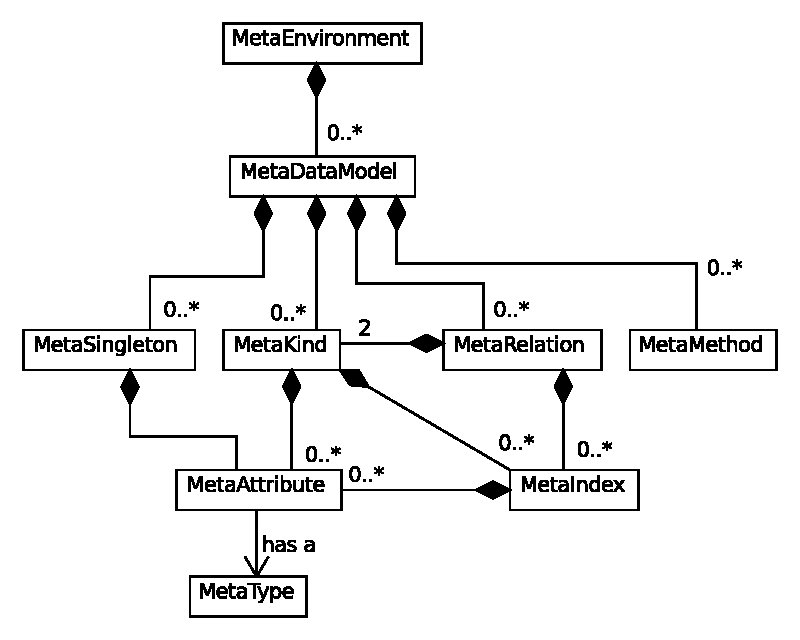
\includegraphics[width=0.75\textwidth]{img/metaModel.pdf}
%	\caption{The class diagram of the meta model is the %abstract syntax of the data model definition.}
%	\label{fig:metaModel}
%\end{figure}


\subsubsection{Kinds and Entities}

\begin{wrapfigure}{r}{0.4\textwidth}

	\begin{center}
		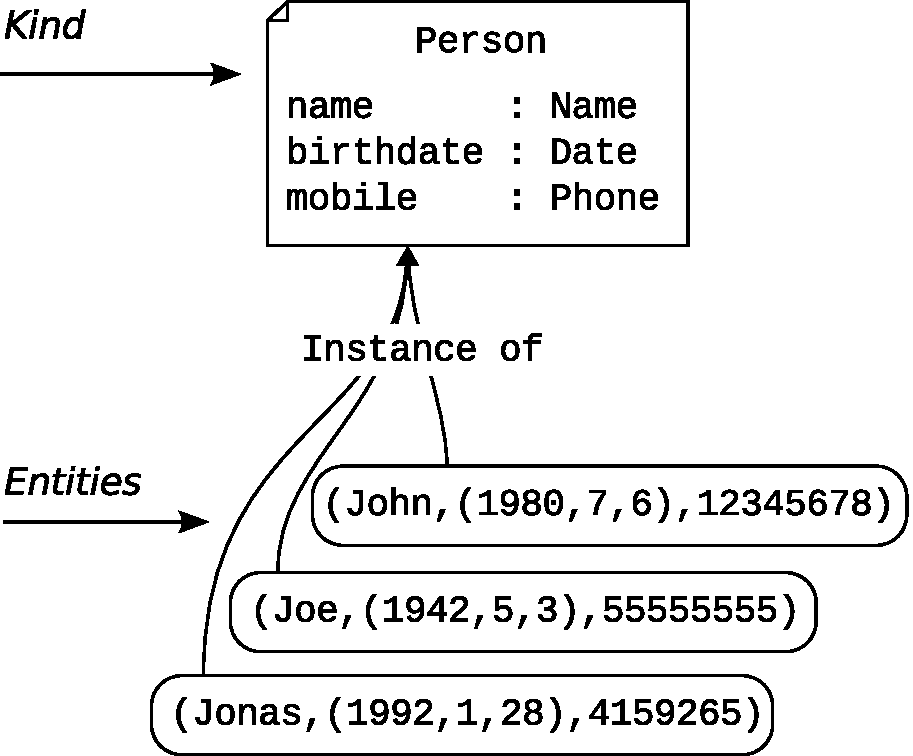
\includegraphics[width=0.4\textwidth]{img/kindAndEntities.pdf}
	\end{center}
	\caption{Kinds describe and contain entities, having certain attributes.}
	\label{fig:kindAndEntities}
\end{wrapfigure}

In EDMA a \emph{kind} \nomenclature[kind]{Kind}{A kind consists of a name and a set of attributes. An instance of a kind is called an entity. For example, a kind could be Person, with the attributes name, birth date and phone number. An entity of this kind could be (John, (1980, 3, 5), 31415926).}is
both a data type and a container of all instances of that type. A
kind has a set of \emph{attributes}\nomenclature[attribute]{Attribute}{A name and a value domain. An example could be "age" in the value domain "PositiveInteger", which is comparable to a variable "age" of type "uint". Attributes are either optional or mandatory, and mutable or immutable.},
where each attribute has a name and a value domain. An \emph{entity\nomenclature[entity]{Entity}{A set of values, conforming to a certain kind. }}
is an instance of a kind. As an example we could have a person kind
with attributes like name, gender, birth date, email and phone number.
A person entity would then contain a value for each of the attributes
in the person kind. Each attribute in a kind can be either mutable
or immutable. If it is immutable then a value for the attribute is
set upon creation of an entity, but this value can never change throughout
the lifetime of the entity. An attribute can be optional, which means
that the value corresponding to that attribute may be \emph{null}.
All kinds in EDMA have an attribute called ID, which is a positive
integer that uniquely identifies each \emph{entity} in the kind.


\subsubsection{Relations and Connections}

Assume that we have a person kind and a course kind, and we want to
be able to express that a person is a student on a course. In EDMA
we call this a \emph{relation\nomenclature[relation]{Relation}{A connection between two kinds. If a relation exists between kinds A and B, entities of A and B can be connected. For example, a relation can exist between kinds Course and Student, which means that an entity of course (eg. (Programming, 2012)) can be connected to a Student (eg. (John Doe, 1984, +4531415926)).}}
between the person kind and the course kind. When there is a \emph{relation}
between the person kind and the course kind, it is possible to make
a \emph{connection} between a specific person entity and a specific
course entity. A \emph{relation} is both a description of possible
\emph{connections} between entities and a container for these \emph{connections}.

\begin{figure}[h]
	\centering
	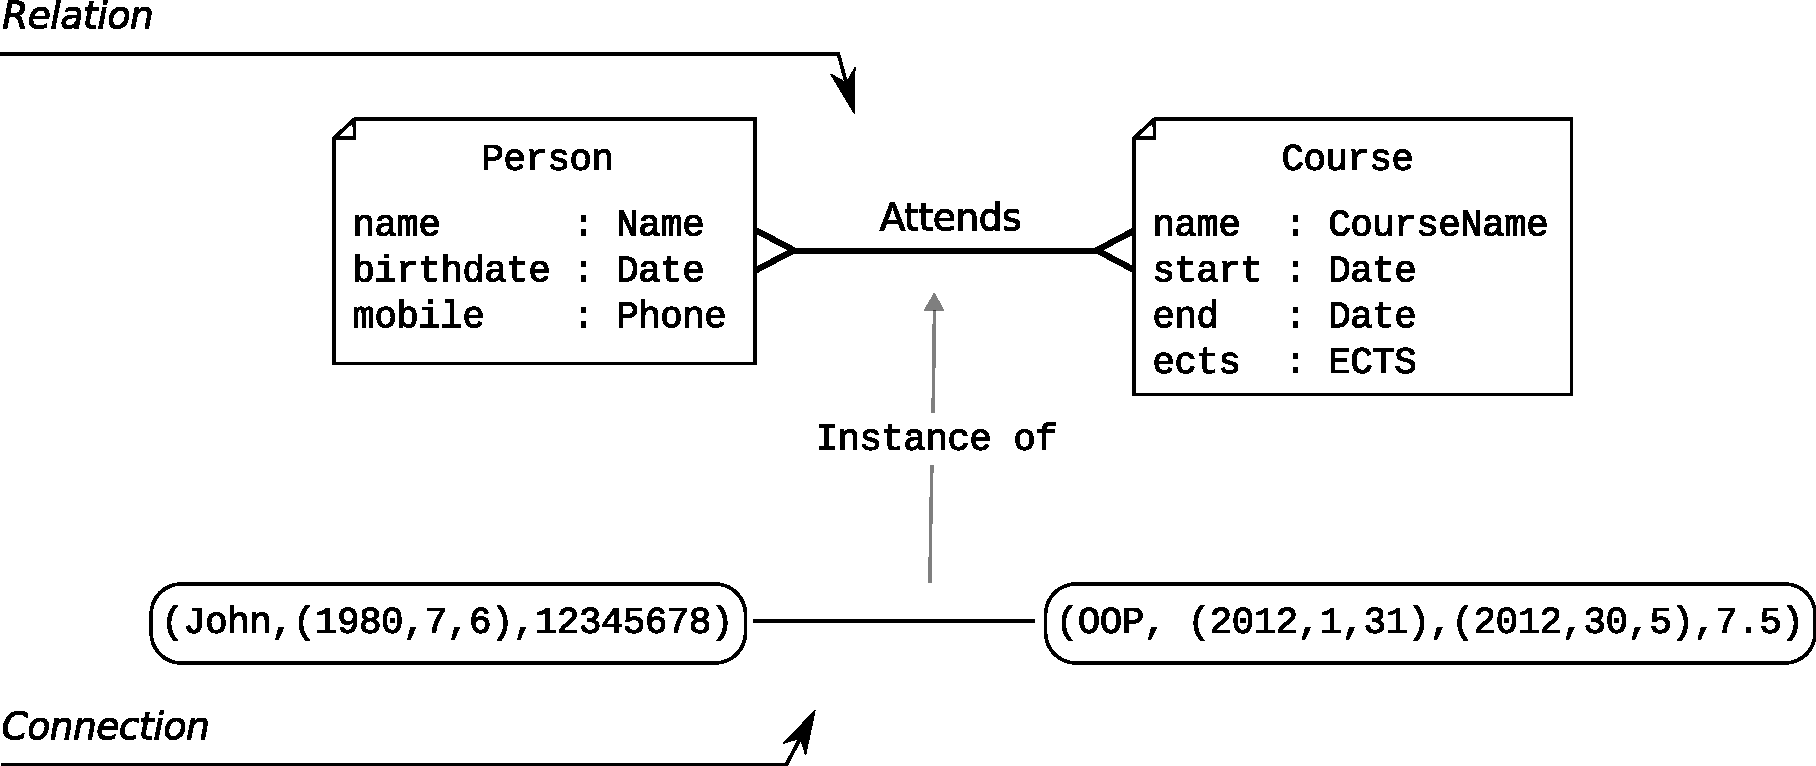
\includegraphics[scale=0.4]{img/relationAndConnection.pdf}
	\caption{A relation between two kinds makes it possible to \emph{connect} entities of those kinds.}
	\label{fig:relationAndConnection}
\end{figure}


\subparagraph{Roles}

A \emph{relation} always has two participants, which we can call A
and B. Both A and B are defined by a \emph{kind} and a \emph{role}.
The reason for having roles is that we can have different relations,
which involve the same kinds, in which case we use the roles to distinguish
them. In the example with the Person kind and the Course kind, we
could have two different relations between them: One that represents
students that are enrolled on the course, and one that represents
teachers that teach the course. To distinguish the two different \emph{relations},
the role of the person would be \emph{student} in the one relation,
and \emph{teacher} in the other. 

\begin{figure}[h]
	\centering
	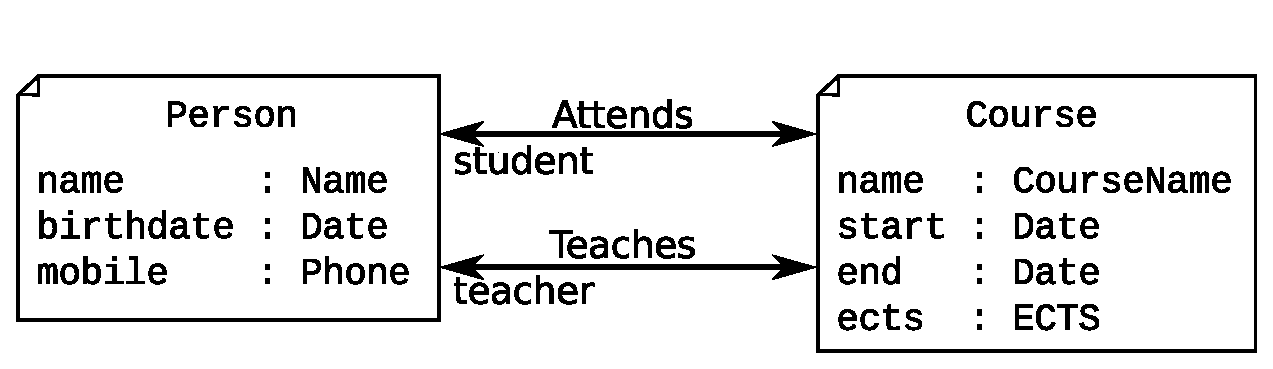
\includegraphics[width=0.75\textwidth]{img/relationRoles.pdf}
	\caption{A Relations between kinds can have roles. This figure shows two relations between the kinds Person and Course. In the first relation, named Attends, the first participant is the Person kind, with the role Student. In the second relation, Teaches, the Person has the role Teacher. In both Relations the second participant is the Course kind with the implicit role course.}
	\label{fig:relationRoles}
\end{figure}

It is also possible to have relations, where both the kind and the
role would be the same for A and B. An example could be a friendship
relation, where the kind is person and the role is friend for both
A and B, this type of relation we call a self-relation. If we have
a relation where A and B has the same kind, but different roles, then
it is not a self relation. An example of this could be where A and
B both are persons, but where the role of A is parent and the role
of B is child. In a self-relation, the order of the participants are
irrelevant, so if we have person a and person b, then ``a is friends
with b'' is the same as ``b is friends with a'', but there is a
difference between ``a is parent of b'' (or ``b is child of a'')
and ``b is parent of a'' (or ``a is child of b'').


\subparagraph{Multiplicities}

We also distinguish between many-to-many, many-to-one and one-to-one
relations (we do not have a one-to-many relation as this is the same
as a many-to-one where A and B are switched). It is worth to notice
that a many-to-one self-relation does not make any sense, so this
leaves us with five different types of relations:
\begin{enumerate}
\item Many-To-Many (MTM)
\item Many-To-Many-Self (MTMS)
\item Many-To-One (MTO)
\item One-To-One (OTO)
\item One-To-One-Self (OTOS)
\end{enumerate}
So, a relation in EDMA contains the following information: a name,
the kind of A, the role of A, the kind of B, the role of B, the type
of the relation (one of the five types above). If a role is not defined
on one of the participants, the role is set to the same as the name
of the participating kind. For example, in the relations shown on
Figure~\ref{fig:relationRoles}, the role of the Course is simply
``course''. In the five relation types above, \emph{many} actually
means \emph{0 or more} and \emph{one} actually means \emph{0 or 1}.

A \emph{connection} is an instance of a relation and can be thought
of as a set of pairs of ids (a, b). Each element in the set represents
the connection between an entity from kind A and an entity from kind
B with the ids a and b respectively. In a self-relation (a, b) is
the same as (b, a).


\subparagraph{Extension}

\begin{wrapfigure}{r}{0.3\textwidth}
	\vspace{-0.415cm}
	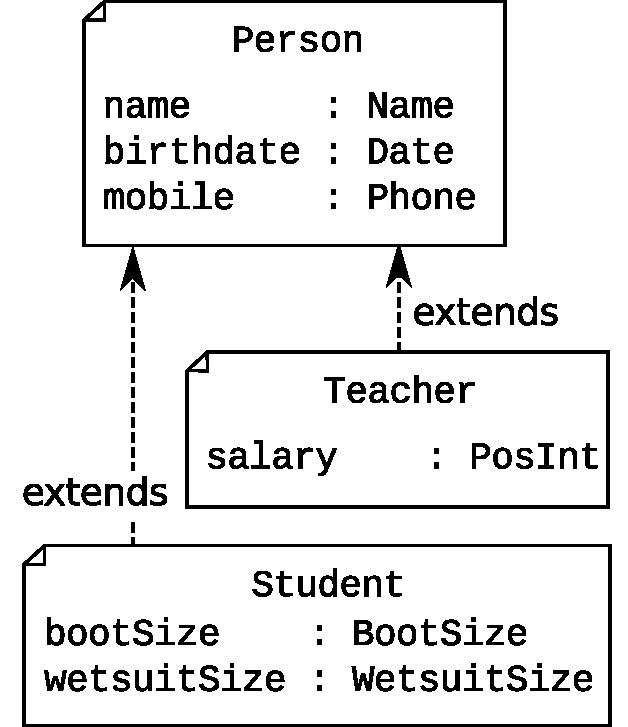
\includegraphics[width=0.3\textwidth]{img/kindExtension.pdf}
	\caption{Here, Student and Teacher extends Person, adding extra attributes.}
\end{wrapfigure}

There is actually a sixth relation type, which we call \emph{extension}.
An extension between kinds is a 1-to-(0 or 1) relation between two
different kinds. As an example we could have a kind, Person, and another
kind, Student, which extends Person. This means that every student
is also a person, so in order to create a new student, you would need
to provide an already existing person, that is not already a student.
We could also have another kind, Teacher, that also extends Person.
Then every teacher would also be a person, and a person could be both
a teacher and a student, or only one of them, or neither. In our running
example with the diving school, we have shown the kinds Student and
Teacher that both extend the kind Person.


\subsubsection{Indexes}

In EDMA indexes are used for two different purposes: To enforce uniqueness
of certain attributes within all entities of a kind, and to gain fast
and easy access to certain entities, or sets of entities. Indexes
can either be declared on a kind, in which case they cover all entities
of that kind, or they can be declared on a relation, in which case
they cover only sets of entities, that are grouped by that relation.
EDMA supports three types of indexes: \emph{Unique}, \emph{Equal}
and \emph{Compare}. 


\subparagraph{Unique index}

The \emph{unique index} is used to enforce uniqueness of one attribute
or a combination of attributes within all entities of a kind, or within
sets of entities grouped by a relation. The unique index also gives
a fast search mechanism using the attributes in the index. 

As an example, we could have a Person kind with attributes \texttt{firstName}
and \texttt{lastName}. If we declared a \emph{unique} index on (\texttt{firstName},
\texttt{lastName}) in the person kind, then this would enforce the
uniqueness of the combination of first name and last name, across
all person entities. If we were to create a person with a name that
were already taken, we would get an exception. If instead we declared
the index on a relation that connects persons and courses, then we
could have two or more persons with the same name, but they could
not attend the same course, because the index would cover every set
of persons connected to the same course.

In the example with the unique index on first name and last name,
it is very fast to get access to a specific person entity, given that
you know the first name and last name.


\subparagraph{Equals index}

The \emph{equal index} does not enforce any constraints, but are used
to get fast access to sets of entities, where the involved attributes
are equal to a certain value. As an example we could have an equal
index on the attribute \texttt{firstName}, making it very fast to
find all entities with a specific first name.


\subparagraph{Compare index}

Like the equal index, the\emph{ compare index} does not enforce any
constraints, but are only used to speed up certain searches among
entities. With a compare index, it is not only possible to search
for entities where the involved attributes are equal to some value.
It is also possible to find sets of entities, where the involved attributes
are less than a given value, greater than a given value or within
a range. The compare index uses the natural order of the value domains.


\subsubsection{Singletons}

Singletons are very similar to kinds, except that they contain exactly
one entity. If a singleton defines non-optional attributes, the values
for these attributes most be provided upon creation of the data model
instance. It is worth to note here that singletons are singletons
on the data model \emph{instance} level, not on the data model level.


\subsubsection{Actions and Views}

Kinds and relations make up the structure of the data model. Actions
and views make up the external interface to the data model. Actions
can both read and change the state of the data model instances, views
can only read the state. We call both actions and views \emph{methods}
if we do not need to distinguish between them.

Methods have a set of input and output parameters, each having a name
and a value domain. Both input parameters and output parameters can
be declared optional. Methods also return an error-code. The possible
error-codes are defined in the definition of the method. An error-code
of 0 always means that the method completed successfully and the output
parameters are valid. Any other error-code means that the method could
not complete for some reason and the output parameters are invalid
(meaning that they are all \emph{null}). For actions an error-code
different from 0 also means that the state of the data model is left
unchanged (any changes made by the action before it returns a non-zero
error-code is automatically rolled back).

An example of an action could be one for adding a student to a course.
It would take two input parameters: the ID of the student, and the
ID of the course, and the action would not have any output parameters
except for the error-code. Error-codes would then be defined for situations
where there is no student with the given ID, no course with the given
ID or the student is already assigned to the course. There could also
be an error-code for the situation where the student do not have enough
funding to pay for the course. As seen here the error-codes are dependent
on the business logic for the data model and the user can define any
number of error-codes that seems fit.

An example of a view could be getting the set of all students enrolled
on a specific course. This view would take a course ID as input and
the output would be a list of students. An error-code could be defined
for the situation where there are no course with the given ID.

The actions and views are atomic operations -- they either complete
successfully and return an error-code of zero, or they fail and return
a non-zero error-code, in which case no changes are made to the state
of the data model instance.


\paragraph{\label{sub:Transactions}Transactions}

Although we have taken an object oriented approach on the data models
and on a high level of abstraction see a data model instance as just
an object with synchronized methods, we want to elaborate a bit more
on the transactional model behind the scene.

In this subsection we will now switch to a more database oriented
terminology and call the methods on a data model instance \emph{transactions}.

The illusion of complete mutual exclusive access to a data model instance,
in database terminology, is the isolation property of the ACID (Atomicity,
Consistency, Isolation and Durability) properties.

Although some object oriented languages supports methods to obtain
isolation in multi-threaded environments, like the synchronize keyword
in Java, they do not incorporate support for the other ACID properties
in the core language.

This is something that we want to address in EDMA, therefore we will
now go through each of the ACID properties and discuss how they will
be handled in the example runtime. 


\subparagraph{Atomicity}

This guarantees that a transaction is executed as an atomic unit,
which means that it either completes successfully or does not change
the state of the data model at all. This property is only relevant
for \emph{actions}, since \emph{views} can never change the state
of the data model anyway. The way this is implemented is through a
rollback functionality. At any stage during the execution of an \emph{action},
if something unexpected happens, or if the action is not able to complete
successful for some reason, it can choose to abort (by returning a
non-zero error-code) and any changes it have already made to the state
of the data model up to this point will be automatically rolled back.

This has been implemented in the example runtime implementation by
defining a small set of six primitive reversible operations that can
be performed on the data model. These are the only operations allowed
on the lowest level, so every execution of an action are broken down
to a sequence of these primitive operations. When an action is executed
these primitive operations are recorded and in the case of a rollback
they can be inverted and played back in a reversed order which will
effectively bring the data model back to the starting state. The set
of primitive operations contains the following six operations:
\begin{itemize}
\item Update an attribute in a singleton
\item Create a new entity
\item Delete an entity
\item Update an entity
\item Create a new connection in a relationship
\item Delete an existing connection in a relationship
\end{itemize}
Each of these operations contains just enough information to be able
to perform the reversed operation as well. This means that ``updates''
contains both the old and the new values and ``deletes'' contains
information about the deleted item so it can be re-created. These
sequences of primitive operations are also the basis for the persistence,
which will be discussed later.


\subparagraph{Consistency}

When we say that the data model is in a consistent state, we mean
that all consistency rules set up by the designer of the data model
is respected in this state. Every \emph{action} must guarantee that
if it starts its execution with the data model in a consistent state,
then the data model is also in a consistent state upon successful
completion of the \emph{action. During }the execution of the action,
it is allowed for the data model to be in a non-consistent state.
In EDMA it is therefore considered as an \emph{error} in the programming
of an \emph{action} if it can move the data model from a consistent
state to a non-consistent state.

At the time of writing this document there have not been incorporated
a way to define consistency rules for EDMA data models (except for
the value domain system and the unique index). But this would be an
obvious extension of EDMA.

Depending on number and type of consistency rules it can be very slow
to test the consistency of a data model. Therefore it can be a good
idea to split consistency checks into different categories of checks
that only looks at parts of the data model. For example we could define
a kind consistency to only concern the attributes of an entity kind.
This consistency would only have to be checked when a new entity is
created or an existing entity is updated. Then we could define a relationship
consistency that would concern a specific relationship, this would
then have to be checked whenever a new connection is made, a connection
is removed or if any of the participating entities are updated. But
there could also be more complex consistency rules that would have
to look at larger parts of the data model and these would be difficult
to generalize about and therefore they would have to be checked after
each update of the data model. Because of the potential large impact
that consistency checks can have on the performance, we would consider
them as part of a debugging process and there should be a possibility
to turn them off when there is enough confidence in the implementations
of the actions and better performance is needed. 

It would be quite easy to implement a complete consistency check that
could be run after each successfully executed action, but we think
that a more general consistency and trigger framework is much more
desirable and therefore we have hesitated to implement this simple
solution.


\subparagraph{Isolation}

The isolation property says that during the execution of a transaction,
this transaction may not see any changes to the state of the data
model caused by other transactions. Or in other words: during the
execution of a transaction it must seem to that transaction that it
is the only transaction running at that time.


\subparagraph{Durability}

Traditionally durability means that once a transaction is committed
it stays so, even in the event of a system failure. As we see it,
there are at least two problems with this formulation:
\begin{enumerate}
\item It is not clear what is covered by the term ``system failure''.
Is it enough that data is stored on the local hard drive or should
it be stored on several different hard drives located in different
cities or even on different continents? No matter how secure the data
is stored it is always possible to think of some (maybe very unlikely)
event that would wipe out all the data. In the EDMA example runtime
implementation we have solved this by having an interchangeable persistence
module with a simple interface that handles the persistence strategy.
So in EDMA we define data to be persisted whenever the persistence
module say so.
\item It is not perfectly clear if this formulation covers both updates
and queries on the database. For \emph{actions} it is clear that when
they return from execution successfully, then any changes they have
made to the state of the data model should already be persisted. But
we think that it should also cover \emph{views}, so whenever a view
returns from execution, then any data seen by that view must be persisted.
\end{enumerate}
So in EDMA we will reformulate the durability property to something
that is a bit more clear on what we mean exactly: 

Durability is the property ensuring that: When a transaction (both
views and actions) has returned successfully from its execution, the
state of the data model known by the transaction at the end of the
execution, must be persisted successfully.


\subparagraph{Transaction Model}

Since we want to abstract a data model instance to an object with
synchronized methods that operates on an internal state, we have chosen
a flat transaction model, where the transaction begins upon entering
the method execution and ends upon exiting the method execution. In
this way the end user of EDMA will never have to think about transactions
or write transaction begin and end declarations.


\subsubsection{Data Models}

A data model can be seen as a class with an internal, encapsulated
state and an external interface. There can be many instances of the
same data model, just as there can be many instances of a class. A
data model instance also defines a transactional context, meaning
that the internal state of the instance is under transactional control,
but it is not possible to make transactions that span more than one
data model instance.

In a large software project there could be several different data
models covering different areas of the business model and there could
be several instances of each data model. 

The value domain system is the infrastructure that EDMA provides to
transport information between different data model instances. Since
all values in the value domain system are immutable and self-contained
it is easy to seamlessly distribute the data model instances on different
physical machines.


\subsubsection{Environment}

An environment is a collection of data models that ``speak the same
language''. By this we mean that the environment defines a set of
common value domains that the data models use in their methods. Each
data model can also define local value domains that are only relevant
in dealing with that specific data model.

Both the common value domains and the local value domains are available
to applications that uses the data models in the environment.
